\documentclass{article}

\usepackage[brazil]{babel}
\usepackage[utf8]{inputenc}
\usepackage[T1]{fontenc}% optional T1 font encoding
\usepackage[%
    colorlinks=true,
    pdfborder={0 0 0},
    linkcolor=red
]{hyperref}
\usepackage[all]{hypcap}
\usepackage{amsmath}
\interdisplaylinepenalty=2500
\usepackage{graphicx}
\usepackage[cmintegrals]{newtxmath}
\usepackage{cite}
\usepackage{listings}
\usepackage{hyperref}
\usepackage{indentfirst}
\usepackage{siunitx}
\usepackage{textgreek}
\usepackage[portuguese,linesnumbered,ruled]{algorithm2e}
\usepackage{multirow}
\usepackage{anysize}
\usepackage{float}
\usepackage{aliascnt}
\newaliascnt{eqfloat}{equation}
\newfloat{eqfloat}{h}{eqflts}
\floatname{eqfloat}{Equation}

\newcommand*{\ORGeqfloat}{}
\let\ORGeqfloat\eqfloat
\def\eqfloat{%
  \let\ORIGINALcaption\caption
  \def\caption{%
    \addtocounter{equation}{-1}%
    \ORIGINALcaption
  }%
  \ORGeqfloat
}

\begin{document}

\title{Diodos e Fontes de Tensão Contínua}
\author{Bianca Yoshie Itiroko - 164923, Luiz Eduardo Cartolano - 183012, Seong Eun Kim - 177143 \\ EE534 - Turma Y - Grupo 2}
\date{Setembro de 2018}

\maketitle

\begin{abstract}
Esse experimento tem como objetivo estudar o funcionamento do transistor \emph{MOSFET}, por meio da análise de seu comportamento nas diferentes regiões (corte, saturação e triodo) e aplicá-lo na construção de um amplificador de áudio. Através dele, calculou-se $V_{th}$ de $1,4V$ e verificou-se um ganho de tensão de aproximadamente $8$.
\end{abstract}

\section{Introdução}
O transistor \emph{MOSFET}, é o tipo mais comum de transistores de efeito de campo em circuitos digitais ou analógicos. Ele é composto de 4 terminais, Dreno, Fonte, Porta e Substrato. São normalmente compostos de um canal de material semicondutor de tipo N (NMOS) ou de tipo P(PMOS). Geralmente o semicondutor escolhido é o silício, mas alguns fabricantes, principalmente a IBM, começaram a usar uma mistura de silício e germânio (SiGe)

O \emph{MOSFET} possui uma série de aplicações práticas que pode-se observar no nosso cotidiano, eles podem ser usados como \emph{switches}, em circuitos amplificadores de banda larga, seguidores de fonte ou ainda em osciloscópios.

Neste experimento, será estudado, com mais detalhes, as características do \emph{MOSFET}, e também, o seu uso no projeto de um circuito amplificador de áudio. Busca-se entender as relações entre o comportamento das tensões V$_{GS}$ e V$_{DS}$, e como elas se comportam com relação a corrente I$_D$. 

\section{Procedimentos}
Para a realização dos experimentos propostos, foram utilizados os seguintes componentes e ferramentas: Osciloscópio digital de dois canais, gerador de ondas/funções, fonte de tensão contínua, cabos com plugs banana e coaxial, multímetro digital, placa de contatos, transistores \emph{BSS100}, um resistor de potência de $100\Omega (5W)$, capacitores de $680nF$ e resistores de $47\Omega$, $55\Omega$, $68\Omega$, $82\Omega$, $240k\Omega$, $270k\Omega$, $1M\Omega$ e $3,9M\Omega$.

A primeira parte consiste na familiarização dos alunos com o \emph{MOSFET}, para isso montou-se o circuito que pode ser observado na Figura \ref{fig:circ1}. Nesta etapa buscou-se encontrar a tensão "limiar" do transistor, V$_{TH}$. E depois, fixando um valor para V$_{GS}$, fez-se medições de V$_{DS}$, a fim de determinar a curva V$_{DS}$ x I$_D$. Também nessa etapa buscou-se encontrar características básicas do transistor. Um detalhe importante ao qual deve-se atentar nesse momento é a presença do resistor de potência, e também a tensão de V$_{CC}$ (corrente contínua), já que em valores muito altos ela pode queimar o transistor.

Na segunda etapa do laboratório, buscou-se estudar uma das aplicações práticas do transistor. Para isso, projetou-se um amplificador de áudio, como o que pode ser observado na Figura \ref{fig:circ2}. Para isso, dimensionou-se um resistor de carga, R$_D$ de $82\Omega$, um resistor R$_1$ de $3,9M\Omega$ e um R$_2$ de $1M\Omega$ (valores teóricos). Além dos capacitores e do transistor abordados no primeiro parágrafo. Novamente, deve-se reiterar o cuidado com a tensão contínua V$_{CC}$ e com o posicionamento dos canais do transistor no circuito, afinal, esses pequenos detalhes são fundamentais para garantir a integridade do circuito.

\section{Discussão}
Na primeira parte do experimento, montou-se o circuito da Figura \ref{fig:circ1} buscando determinar a tensão limiar do \emph{MOSFET}. Para tal, aumentou-se a tensão de $V_{GS}$ aos poucos afim de descobrir em que tensão a corrente começaria a ser conduzida. Obteve-se um valor entre $1,3V$ e $1,4V$, sendo que a inexatidão dessa medição pode ser atribuída ao fato de que a fonte de tensão não tinha muitas casas decimais, de forma que o valor era arredondado.

A fim de obter dados para uma análise da entrada e da saída do \emph{MOSFET} utilizou-se o gerador de funções (utilizando a função dente-de-serra) e o osciloscópio. Fixou-se uma tensão de alimentação em $12V$, um offset de $3V$ e variou-se a tensão de $V_{GS}$. Assim, obteve-se o Gráfico \ref{fig:mos_vds_vgs}, onde pode-se observar o comportamento do transistor à medida que o $V_{GS}$ varia: quando temos tensões menores do que $V_{TH}$, não há condução de corrente e portanto pudemos concluir que o mesmo estaria na região de corte (Figura \ref{fig:mos_corte_osc}). Logo após $V_{TH}$, é perceptível que a curva de saída tem comportamento próximo ao de uma parábola (Figura \ref{fig:mos_sat_osc}), esse comportamento, se dá, muito provavelmente, pela ocorrência de um "estrangulamento" no canal do dreno, reduzindo a corrente que passa por lá, e desse modo, a tensão de saída se modifica em relação a de entrada, e pode-se concluir que estamos na região de saturação. Por fim, quando V$_{GS}$ ultrapassa algo em torno de $2,5V$, o sinal de saída volta a ser constante em relação à entrada (Figura \ref{fig:mos_tri_osc}), e neste caso, ele encontra-se na região de triodo. Um gráfico com as três regiões indicadas pode ser encontrado na Figura \ref{fig:regioes}.

Visando construir a relação corrente x tensão para o transistor, fixou-se valores constantes de $V_{GS}$, inicialmente $2V$, depois $1V$ e por fim $4V$. E, alterou-se, gradativamente, a tensão de alimentação $V_{CC}$, ao mesmo tempo que medíamos a tensão de $V_{DS}$, construindo as tabelas observadas (Tabelas \ref{table: 1}, \ref{table: 2} e \ref{table: 3}).

A partir dos dados obtidos nas Tabelas \ref{table: 1}, \ref{table: 2} e \ref{table: 3}, foi possível montar o gráfico para o \emph{MOSFET} nas regiões de corte (V$_{GS}$ = 1V, Figura \ref{fig:mos_corte}), saturação ((V$_{GS}$ = 2V, Figura \ref{fig:mos_sat}) e triodo (V$_{GS}$ = 4V, Figura \ref{fig:mos_tri}). Da literatura, \cite{Sedra2004}, pode-se chegar para o transistor em saturação, na Equação \ref{eq:k}, que permite calcular o valor da constante k, para o qual chegamos em 0,034 $A/V^2$. A partir do valor de K, é possível calcular o parâmetro da modulação de tamanho de canal ($\Lambda$), usando a Equação \ref{eq:lambda}, para o qual obtemos um valor 0,028 1/V. A partir do parâmetro da modulação de tamanho de canal pode-se também encontrar a tensão de Early ($V_A$) do nosso transistor, mais detalhes podem ser observados em \citeonline{ref:early}, para o qual obtemos 35V.

A fim de comparar os dados encontrados experimentalmente para a corrente no dreno $I_D$, buscou-se obter os valores teóricos para a corrente. Para isso, usou-se \cite{Sedra2004}, de onde encontrou-se as equações para a corrente no dreno para o \emph{MOSFET} nas regiões de saturação e triodo, Equações \ref{eq:corr_sat} e \ref{eq:corr_tri}. A partir delas, e usando os parâmetros anteriormente encontrados, plotou-se os gráficos do \emph{MOSFET} em saturação, triodo e corte, que podem ser observados nas Figuras \ref{fig:mos_sat_teo}, \ref{fig:mos_tri_teo} e \ref{fig:mos_cor_teo}. Comparando os gráficos obtidos com valores teóricos e experimentais, é possível perceber uma pequena diferença. Para a região de corte, por exemplo, os valores experimentais não foram exatamente iguais a zero, o que pode ser causado por falhas na medição de $V_{DS}$. Para a região de triodo, é possível observar que o gráfico experimental começa a se curvar um pouco antes, novamente, uma boa justificativa, seria a baixa precisão das medições feitas com o multímetro. A maior diferença, entretanto, está na região de saturação, o gráfico teórico se mostrou muito mais linear do que o experimental, uma provável razão é o \emph{range} de valores para a corrente, que se mostrou muito mais variado nas medições feitas.

Após as análises, pode-se concluir que a região de atuação do \emph{MOSFET} que melhor funciona como amplificador é a de saturação, uma vez que para as regiões de corte e de triodo tem-se praticamente um comportamento constante, logo não fariam efeito no amplificador.

Para a segunda parte do experimento (circuito da Figura \ref{fig:circ2}), usou-se o valor de $k$ calculado anteriormente e, usando a Equação \ref{eq:gain_mos}, obteve-se o ganho do \emph{MOSFET} ($g_m$). A partir dele, pode-se calcular o valor esperado de $R_1$ e $R_D$ (Equações \ref{eq:calc_R1} e \ref{eq:calc_Rd}), que foram de $245,1 \Omega$ e $5M \Omega$, respectivamente. Dessa forma, usou-se no circuito valores próximos a eles, com R$_D$ de $82 \Omega$ e R$_1$ de $3,9 \Omega$.

Um detalhe importante para o circuito amplificador, é o o desejo por trabalhar no ponto de máxima excursão do circuito, ou seja, aproveitar a maior parte do tempo possível na região de saturação. Para isso, é preciso montar um gráfico como o da Figura \ref{fig:carga}, e calcular o ponto desejado como sendo a metade do caminho entre o ponto em que a curva de carga se encontra com a parábola, e o ponto no qual ela cruza o eixo X.

Aplicando-se uma onda senoidal de $100 mV_{pp}$ e uma frequência de $1kHz$, obteve-se no osciloscópio o gráfico da Figura \ref{fig:mos_amp} e, com base nele, pode-se então concluir que o ganho do amplificador foi de 8 a 9, aproximadamente.

Elevando-se gradativamente o valor da amplitude de entrada, quando chegou-se a $900mV_{pp}$ pode-se notar o sinal de saída apresentou distorções, as quais iam aumentando conforme a amplitude aumentava, como pode-se observar na Figura \ref{fig:mos_dis}.

Ao conectar-se a carga de baixa impedância, no caso um alto falante, o amplificador tem seu ponto de operação alterado devido a quantidade de corrente puxada pelo novo elemento. Agora despolarizado, o ganho de tensão diminui, como pode ser observado na Figura \ref{fig:mos_caixa}.

% MIGUE PARA OS VALORES DAS RESISTENCIAS DA ULTIMA PARTE
Para obter melhores valores de resistências, poderia-se ter calculado o valor real de R$_D$ no experimento da Figura \ref{fig:circ1} e do R$_2$ da Figura \ref{fig:circ2}. Dessa forma, possivelmente obteria-se valores diferentes de I$_D$ e calcularia-se um valor diferente para $k$ (Equação \ref{eq:k}), o que, portanto, mudaria os valores das resistências (Equações \ref{eq:calc_Rd} e \ref{eq:calc_R1}). 

\section{Conclusão}
Neste experimento, buscou-se estudar o funcionamento do transistor \emph{MOSFET} e analisar seu comportamento de acordo com a tensão limiar para seu funcionamento $V_{th}$. Assim, conclui-se que o experimento foi bem sucedido, uma vez que o comportamento do \emph{MOSFET} foi condizente com o valor de $V_{th}$ calculado de $1,4V$. Pelos gráficos citados no decorrer deste relatório foi possível classificar as regiões de atuação do transistor (corte, saturação e triodo).
Tendo isso, verificou-se o funcionamento do circuito como um amplificador e obteve-se o ganho: pelo gráfico gerado, foi possível observar que houve amplificação do sinal em fatores de 8 a 9, que foi de acordo com o esperado.
Utilizando o mesmo circuito numa aplicação prática de um alto falante, pode-se checar o comportamento para o caso de despolarização, em que o ganho de tensão diminui, como foi apontado anteriormente.

\nocite{*}
\bibliographystyle{plain}
\bibliography{references}

\newpage
\section*{Anexos}

\begin{figure}[h!]
    \centering
    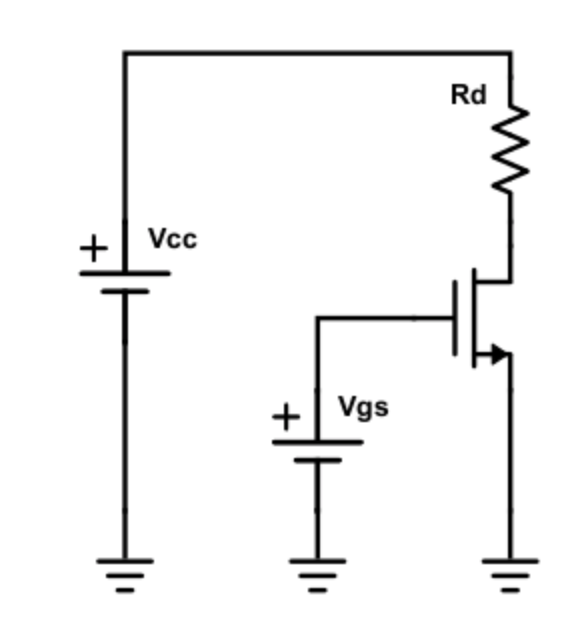
\includegraphics[height=5.5cm]{imgSource/circuito1.png}
    \caption{Circuito para caracterização do transistor MOSFET.}
    \label{fig:circ1}
\end{figure}

\begin{figure}[h!]
    \centering
    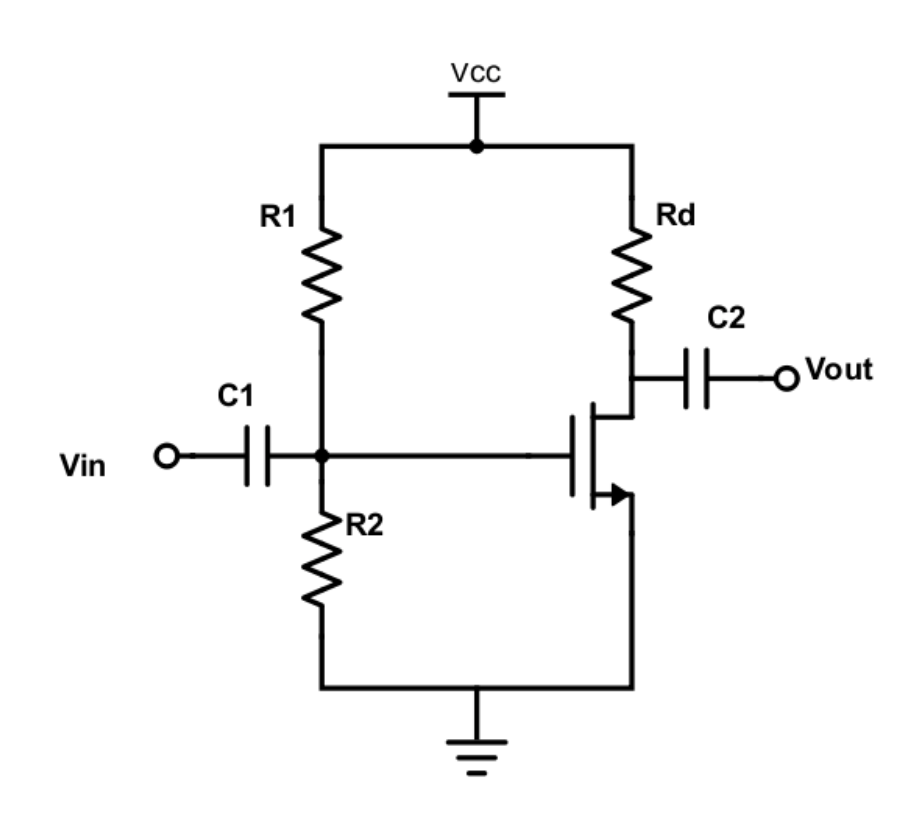
\includegraphics[height=7.5cm]{imgSource/circuito2.png}
    \caption{Circuito amplificador com transistor NMOS.}
    \label{fig:circ2}
\end{figure}

\begin{figure}[h!]
    \centering
    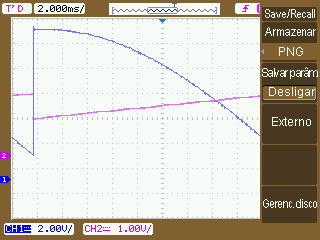
\includegraphics[height=5.5cm]{imgSource/mosfet_sat.png}
    \caption{Comportamento do \emph{MOSFET} na região de saturação.}
    \label{fig:mos_sat_osc}
\end{figure}

\begin{figure}[h!]
    \centering
    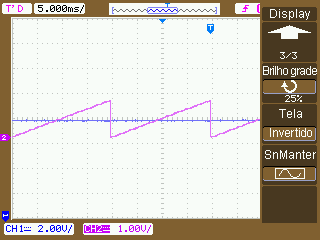
\includegraphics[height=5.5cm]{imgSource/mosfet_corte.png}
    \caption{Comportamento do \emph{MOSFET} na região de corte.}
    \label{fig:mos_corte_osc}
\end{figure}

\begin{figure}[h!]
    \centering
    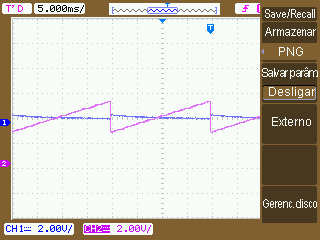
\includegraphics[height=5.5cm]{imgSource/mosfet_tri.png}
    \caption{Comportamento do \emph{MOSFET} na região de triodo.}
    \label{fig:mos_tri_osc}
\end{figure}

\begin{figure}[h!]
    \centering
    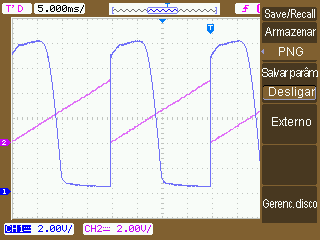
\includegraphics[height=5.5cm]{imgSource/VdsxVgs.png}
    \caption{Comportamento do \emph{MOSFET} sob valores variados de $V_{GS}$.}
    \label{fig:mos_vds_vgs}
\end{figure}

\begin{figure}[h!]
    \centering
    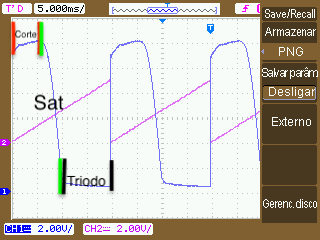
\includegraphics[height=5.5cm]{imgSource/regioes.png}
    \caption{Comportamento do \emph{MOSFET} sob valores variados de $V_{GS}$, com as regiões indicadas.}
    \label{fig:regioes}
\end{figure}


\begin{figure}[h!]
    \centering
    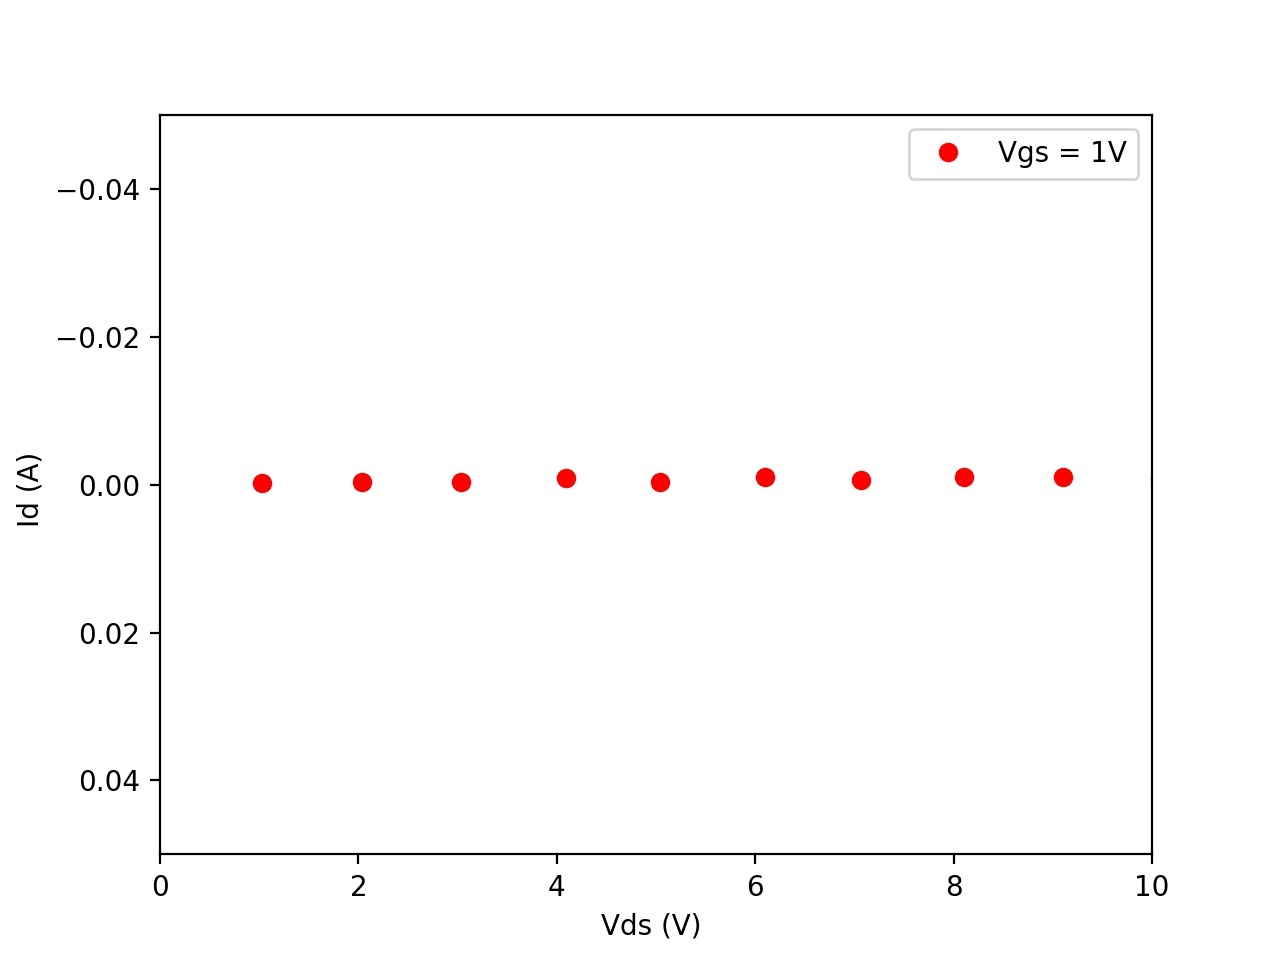
\includegraphics[height=7.5cm]{imgSource/vgs1_exp.jpg}
    \caption{Gráfico obtido experimentalmente de V$_{DS}$xI$_{D}$ para o \emph{MOSFET} na região de corte.}
    \label{fig:mos_corte}
\end{figure}

\begin{figure}[h!]
    \centering
    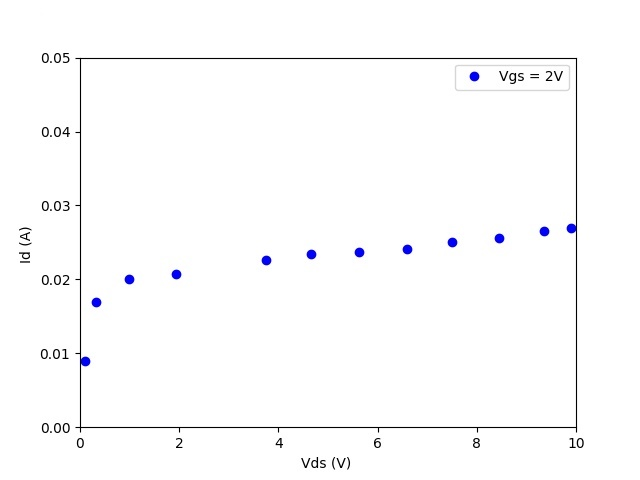
\includegraphics[height=7.5cm]{imgSource/vgs2_exp.jpg}
    \caption{Gráfico obtido experimentalmente de V$_{DS}$xI$_{D}$ para o \emph{MOSFET} na região de saturação.}
    \label{fig:mos_sat}
\end{figure}

\begin{figure}[h!]
    \centering
    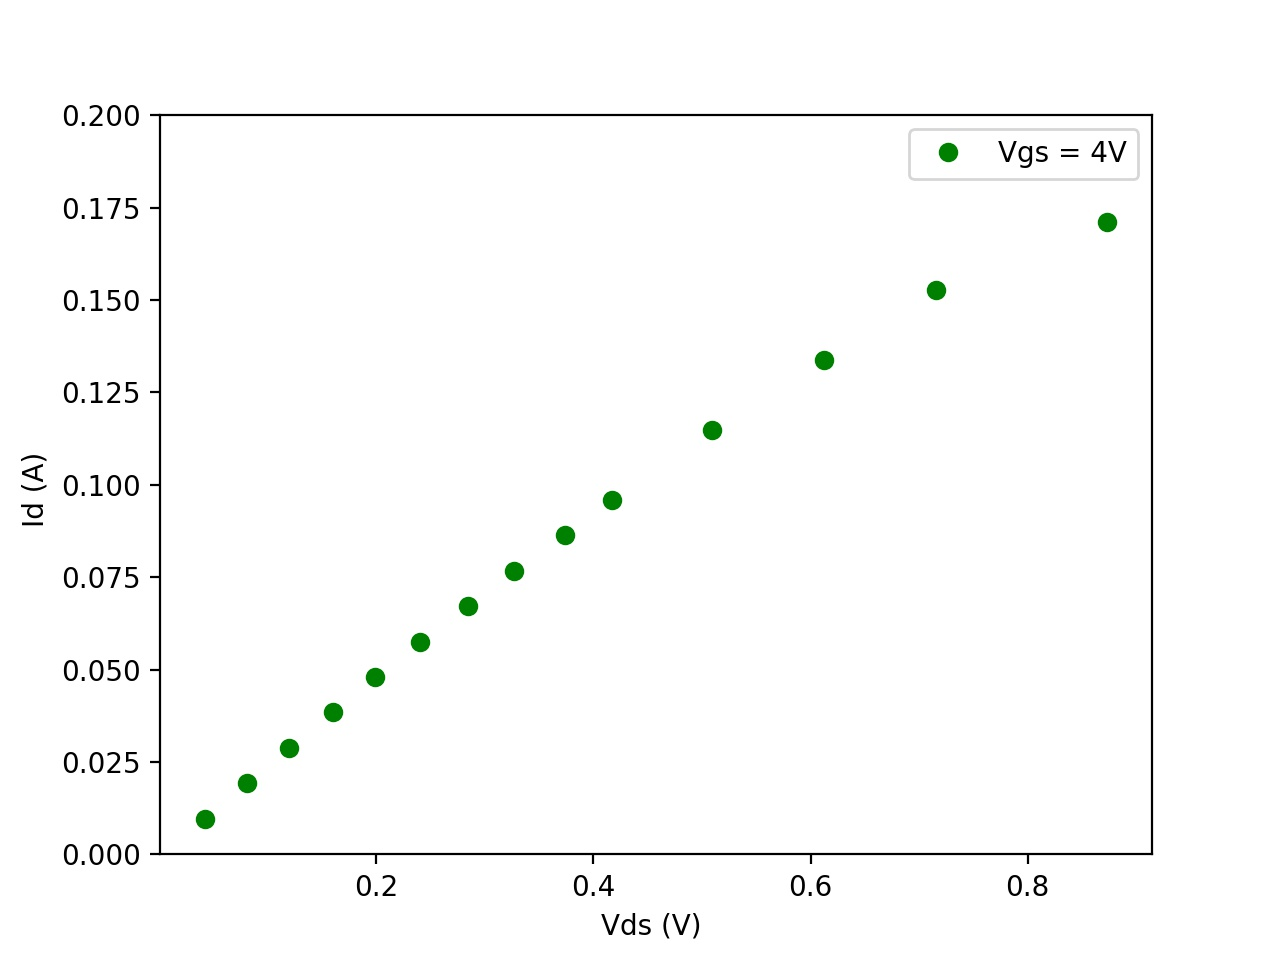
\includegraphics[height=7.5cm]{imgSource/vgs4_exp.jpg}
    \caption{Gráfico obtido experimentalmente de V$_{DS}$xI$_{D}$ para o \emph{MOSFET} na região de triodo.}
    \label{fig:mos_tri}
\end{figure}

\begin{figure}[h!]
    \centering
    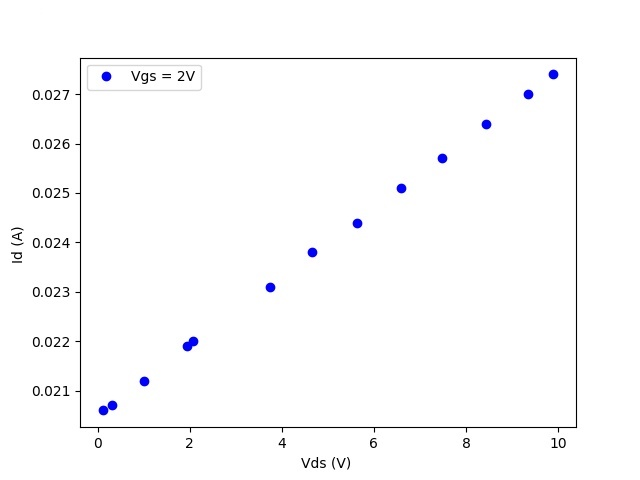
\includegraphics[height=7.5cm]{imgSource/vgs2_teo.jpg}
    \caption{Gráfico teórico de V$_{DS}$xI$_{D}$ para o \emph{MOSFET} na região de saturação.}
    \label{fig:mos_sat_teo}
\end{figure}

\begin{figure}[h!]
    \centering
    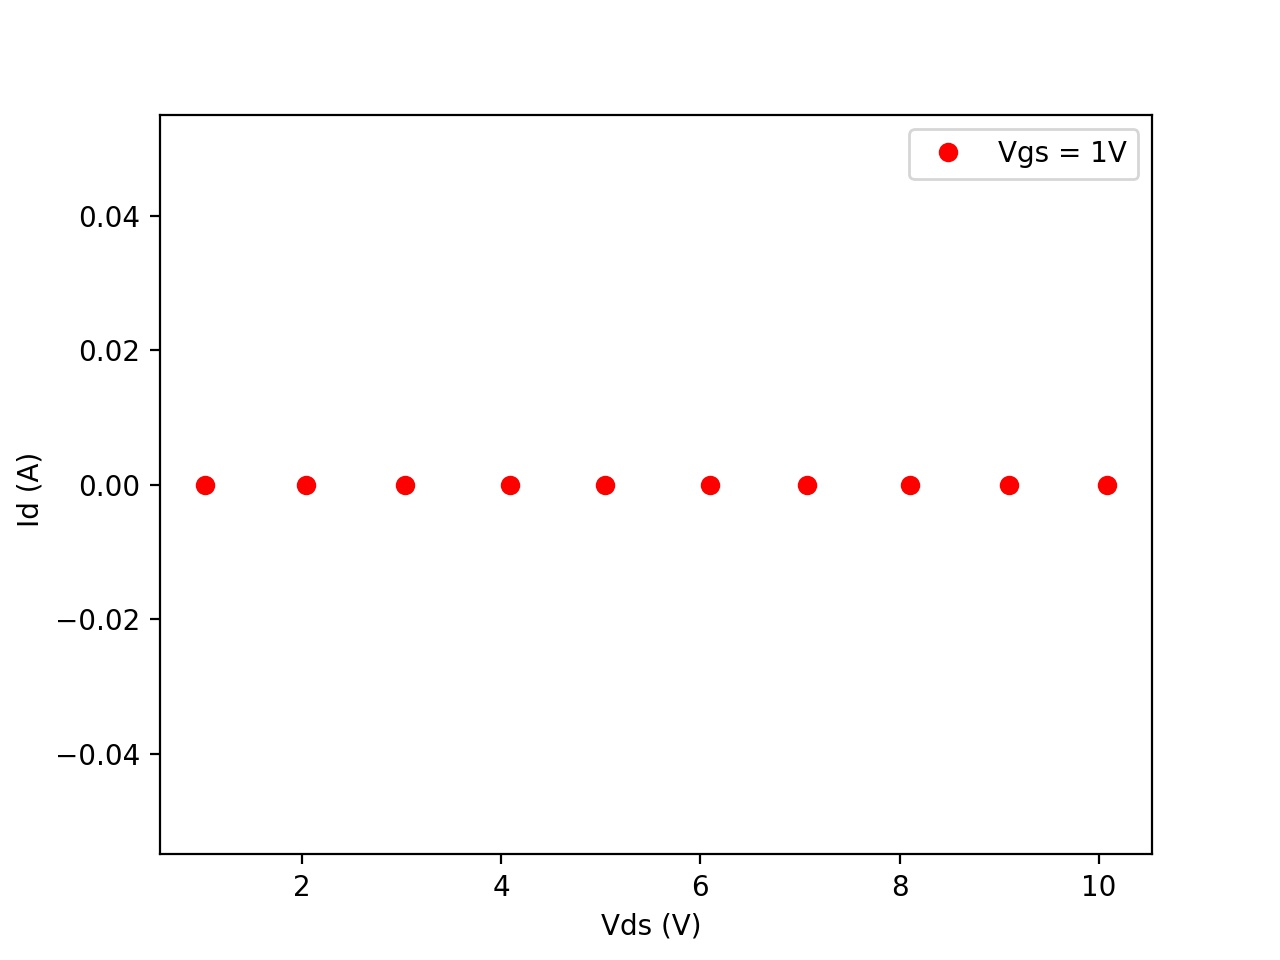
\includegraphics[height=7.5cm]{imgSource/vgs1_teo.jpg}
    \caption{Gráfico teórico de V$_{DS}$xI$_{D}$ para o \emph{MOSFET} na região de corte.}
    \label{fig:mos_cor_teo}
\end{figure}

\begin{figure}[h!]
    \centering
    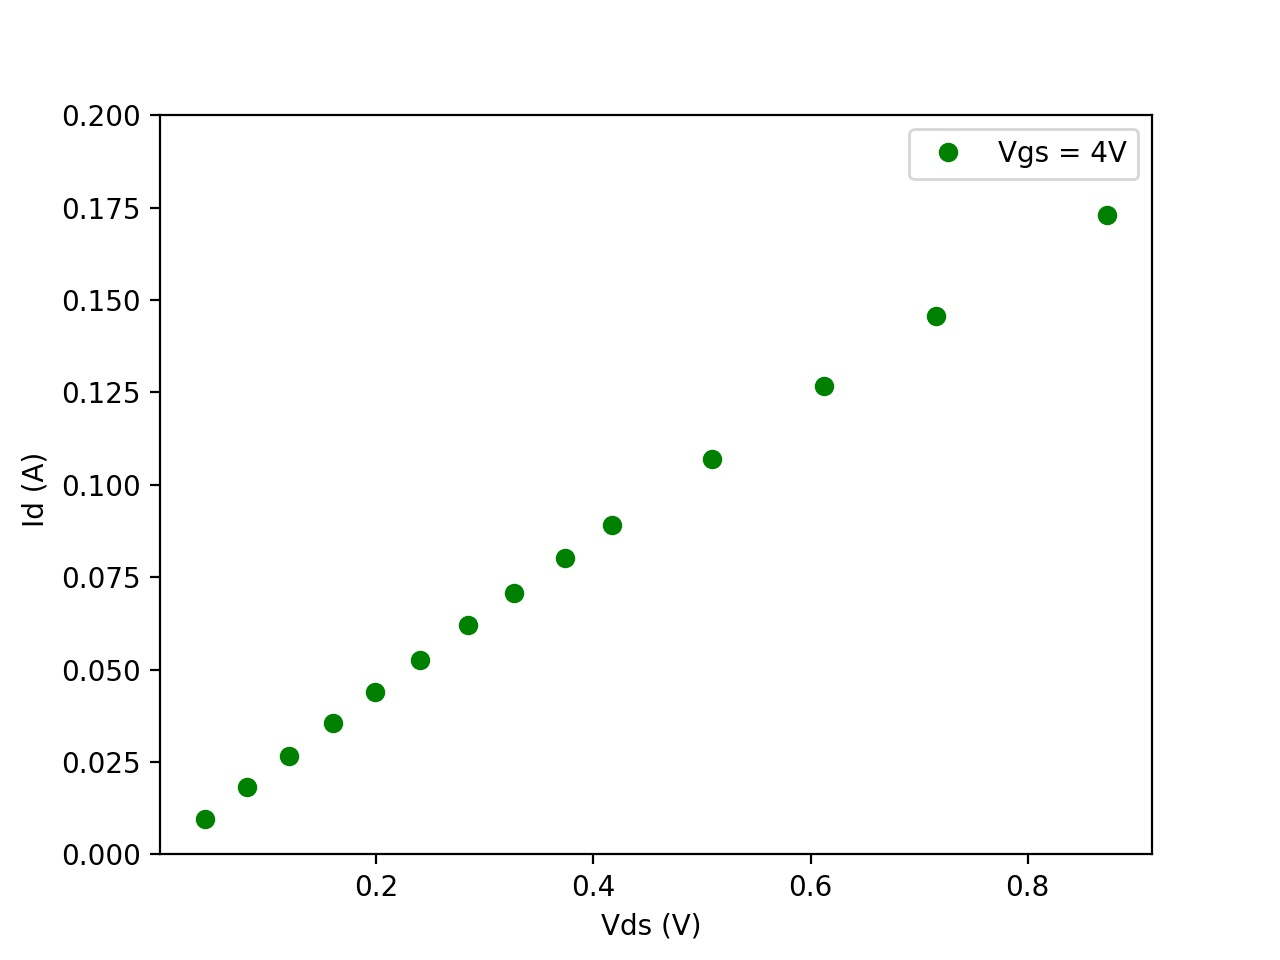
\includegraphics[height=7.5cm]{imgSource/vgs4_teo.jpg}
    \caption{Gráfico teórico de V$_{DS}$xI$_{D}$ para o \emph{MOSFET} na região de triodo.}
    \label{fig:mos_tri_teo}
\end{figure}

\begin{figure}[h!]
    \centering
    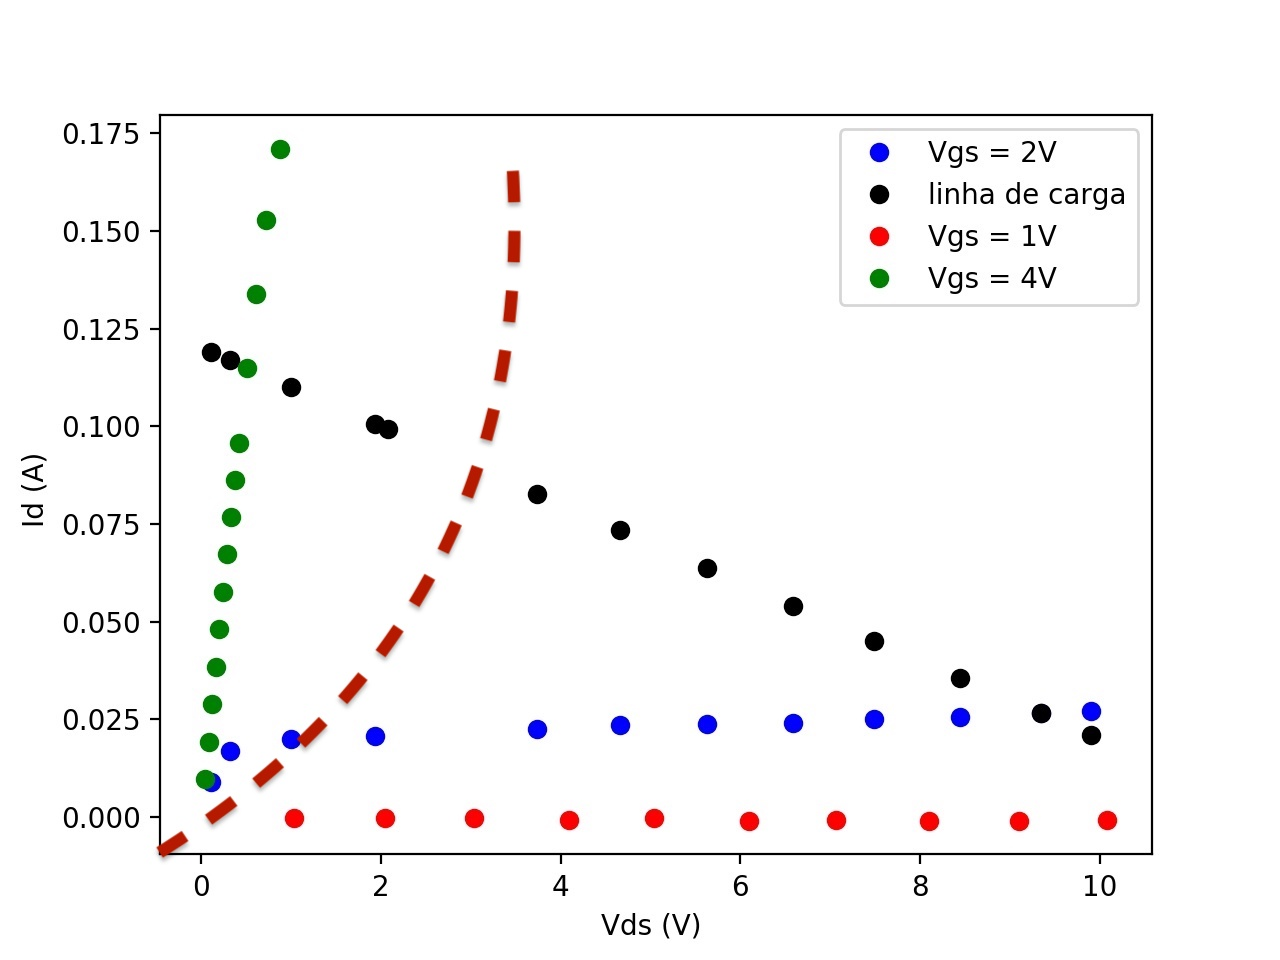
\includegraphics[height=5.5cm]{imgSource/carga.jpg}
    \caption{Gráfico de I$_D$ x V$_DS$, com a curva de carga e a parábola que delimita o limiar entre saturação e triodo traçadas.}
    \label{fig:carga}
\end{figure}

\begin{figure}[h!]
    \centering
    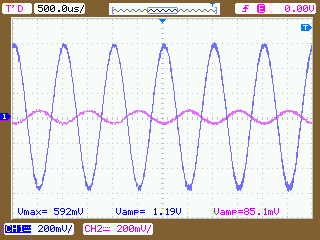
\includegraphics[height=5.5cm]{imgSource/mosfetAmp.png}
    \caption{Comportamento do circuito amplificador classe A.}
    \label{fig:mos_amp}
\end{figure}

\begin{figure}[h!]
    \centering
    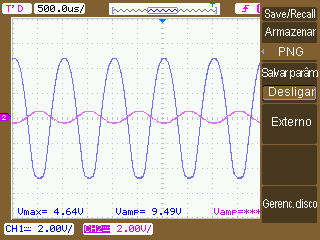
\includegraphics[height=5.5cm]{imgSource/amp900mVpp.png}
    \caption{Início de distorção da curva se saída do circuito amplificador classe A.}
    \label{fig:mos_dis}
\end{figure}

\begin{figure}[h!]
    \centering
    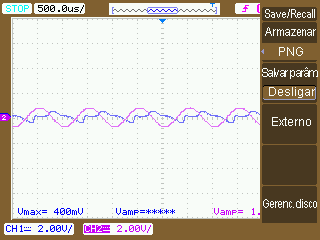
\includegraphics[height=5.5cm]{imgSource/ampCaixa.png}
    \caption{Comportamento do circuito amplificador classe A quando conectado a uma caixa de som.}
    \label{fig:mos_caixa}
\end{figure}

\begin{table}[h!]
    \centering
    \begin{tabular}{|l|l|l|l|}
    \hline
        V$_{CC}$ (V) & V$_{DS}$ (V) & V$_{R}$ (V) & I$_{D}$ (A) \\ \hline
        1 & 0.11 & 0.89 & 0.009 \\ \hline
        2 & 0.31 & 1.69 & 0.017 \\ \hline
        3 & 0.99 & 2.00 & 0.020 \\ \hline
        4 & 1.93 & 2.07 & 0.021 \\ \hline
        5 & 2.07 & 2.93 & 0.029 \\ \hline
        6 & 3.74 & 2.26 & 0.023 \\ \hline
        7 & 4.66 & 2.34 & 0.023 \\ \hline
        8 & 5.63 & 2.37 & 0.024 \\ \hline
        9 & 6.59 & 2.41 & 0.024 \\ \hline
        10 & 7.49 & 2.51 & 0.025 \\ \hline
        11 & 8.44 & 2.56 & 0.026 \\ \hline
        12 & 9.35 & 2.65 & 0.026 \\ \hline
        12.6 & 9.90 & 2.70 & 0.027 \\ \hline
    \end{tabular}
    \caption{Valores de V$_{DS}$ e I$_D$ para V$_{GS}$ de 2V}
    \label{table: 1}
\end{table}

\begin{table}[h!]
    \centering
    \begin{tabular}{|l|l|l|l|}
    \hline
        V$_{CC}$ (V) & V$_{DS}$ (V) & V$_{R}$ (V) & I$_{D}$ (A) \\ \hline
        1 & 1.03 & -0.03 & -0.0003 \\ \hline
        2 & 2.04 & -0.04 & -0.0004 \\ \hline
        3 & 3.04 & -0.04 & -0.0004 \\ \hline
        4 & 4.09 & -0.09 & -0.0009 \\ \hline
        5 & 5.04 & -0.04 & -0.0004 \\ \hline
        6 & 6.10 & -0.10 & -0.0010 \\ \hline
        7 & 7.07 & -0.07 & -0.0007 \\ \hline
        8 & 8.10 & -0.10 & -0.0010 \\ \hline
        9 & 9.10 & -0.10 & -0.0010 \\ \hline
        10 & 10.08 & -0.08 & -0.0008 \\ \hline
    \end{tabular}
    \caption{Valores de V$_{DS}$ e I$_D$ para V$_{GS}$ de 1V}
    \label{table: 2}
\end{table}

\begin{table}[h!]
    \centering
    \begin{tabular}{|l|l|l|l|}
    \hline
        V$_{CC}$ (V) & V$_{DS}$ (V) & V$_{R}$ (V) & I$_{D}$ (A) \\ \hline
        1 & 0.04 & 0.96 & 0.010 \\ \hline
        2 & 0.08 & 1.92 & 0.019 \\ \hline
        3 & 0.12 & 2.88 & 0.029 \\ \hline
        4 & 0.16 & 3.84 & 0.038 \\ \hline
        5 & 0.20 & 4.80 & 0.048 \\ \hline
        6 & 0.24 & 5.76 & 0.058 \\ \hline
        7 & 0.28 & 6.72 & 0.067 \\ \hline
        8 & 0.33 & 7.67 & 0.077 \\ \hline
        9 & 0.37 & 8.63 & 0.086 \\ \hline
        10 & 0.42 & 9.58 & 0.096 \\ \hline
        12 & 0.51 & 11.49 & 0.115 \\ \hline
        14 & 0.61 & 13.39 & 0.134 \\ \hline
        16 & 0.72 & 15.28 & 0.153 \\ \hline
        18 & 0.87 & 17.13 & 0.171 \\ \hline
    \end{tabular}
    \caption{Valores de V$_{DS}$ e I$_D$ para V$_{GS}$ de 4V}
    \label{table: 3}
\end{table}

\begin{eqfloat}
    \begin{equation}
        k = \frac{I_{D,On}}{(V_{GS,On} - V_{TH})^2}
        \label{eq:k}
    \end{equation}
    \caption{Parâmetro K do \emph{MOSFET}}
\end{eqfloat}

\begin{eqfloat}
    \begin{equation}
        \lambda = \frac{I_{D,Sat}}{V_{DS} K (V_{GS} - V_{TH})^2} - \frac{1}{V_{DS}}
        \label{eq:lambda}
    \end{equation}
    \caption{Modulação de tamanho de canal do \emph{MOSFET}}
\end{eqfloat}

\begin{eqfloat}
    \begin{equation}
        I_{D,Sat} = K (V_{GS} - V_{TH})^2(1+\lambda V_{DS})
        \label{eq:corr_sat}
    \end{equation}
    \caption{Corrente do \emph{MOSFET} na região de saturação}
\end{eqfloat}

\begin{eqfloat}
    \begin{equation}
        I_{D,Tri} = K(2(V_{GS} - V_{TH})V_{DS} - (V_{DS})^2 )
        \label{eq:corr_tri}
    \end{equation}
    \caption{Corrente do \emph{MOSFET} na região de triodo}
\end{eqfloat}

\begin{eqfloat}
    \begin{equation}
        g_m = 2 * k * (V_{GS} - V_{TH})
        \label{eq:gain_mos}
    \end{equation}
    \caption{Ganho de tensão do \emph{MOSFET}.}
\end{eqfloat}

\begin{eqfloat}
    \begin{equation}
        R_d = \frac{A_v}{g_m}
        \label{eq:calc_Rd}
    \end{equation}
    \caption{Cálculo de R$_d$}
\end{eqfloat}

\begin{eqfloat}
    \begin{equation}
        V_{GS} = V_{CC} * \frac{R_2}{R_1 + R_2}
        \label{eq:calc_R1}
    \end{equation}
    \caption{Divisor de tensão no V$_{GS}$ para o cálculo de R$_1$.}
\end{eqfloat}


\end{document}
